% Reviewed translation: PDF pages 153--159 / printed pages 139--145.
% The original scan is authoritative; environment headings remain English.
\MathBookSourcePage{153}
\subsection{三角形单元上的高阶逼近}
\label{subsec:primitive-triangle-higher-order}

本小节讨论的有限元空间由 Crouzeix \& Raviart [23] 和 Mansfield [56]
引入. 它们是空间 $\mathcal{P}_1(\kappa)$ 的直接推广. 读者或许会觉得
这些空间很容易理解, 但由于 inf-sup 条件, 对它们的原始分析绝非易事.
幸运的是, Subsection~\ref{subsec:primitive-discrete-inf-sup-methods} 的材料
大大降低了这一困难.

本小节假设 $\Omega$ 是有界平面多边形. 固定整数 $l\geq2$.
设 $\mathcal{T}_h$ 是 $\Omega$ 的一个三角剖分, $\kappa$ 是
$\mathcal{T}_h$ 的任意三角形. 我们仍要构造这样的速度: 其分量为
$l+1$ 次多项式, 且在 $\kappa$ 每条边上的切向分量为 $l$ 次多项式.
但现在多项式次数较高, 对这一问题有一个简单答案: 只需所有 $l+1$
次项在 $\kappa$ 的边上消失; 换言之, 它们必须具有公因子
$\lambda_1\lambda_2\lambda_3$. 更确切地, 用 $\widetilde P_k$
表示 $k$ 次齐次多项式空间:
\[
\widetilde P_k
=\operatorname{span}\{\,x_1^ix_2^{k-i};\ 0\leq i\leq k\,\}.
\]
然后在 $P_{l+1}^2$ 的如下多项式子空间中选取速度 $\mathbf w$:
\begin{equation}\label{eq:primitive-triangle-higher-local-velocity}
\mathcal{P}_l(\kappa)
=\left[P_l\oplus\{\lambda_1\lambda_2\lambda_3\widetilde P_{l-2}\}\right]^2,
\end{equation}
并在 $P_{l-1}$ 中选取压力 $q$. 这导出如下空间选择:
\begin{equation}\label{eq:primitive-triangle-higher-velocity-spaces}
\left\{
\begin{aligned}
W_h&=\{\,\mathbf w\in\mathcal{C}^0(\bar\Omega)^2;
\ \mathbf w|_\kappa\in\mathcal{P}_l(\kappa)
\quad\forall\kappa\in\mathcal{T}_h\,\},\\
X_h&=W_h\cap H_0^1(\Omega)^2,
\end{aligned}
\right.
\end{equation}
\begin{equation}\label{eq:primitive-triangle-higher-pressure-spaces}
\left\{
\begin{aligned}
Q_h&=\{\,q\in L^2(\Omega);
\ q|_\kappa\in P_{l-1}\quad\forall\kappa\in\mathcal{T}_h\,\},\\
M_h&=Q_h\cap L_0^2(\Omega).
\end{aligned}
\right.
\end{equation}

速度 $\mathbf w$ 的自由度选择不再由满足 inf-sup 条件来决定.
因此可以简单地取 $\mathbf w$ 在 $\kappa$ 的边上与 $P_l$ 对应的值,
以及在 $\kappa$ 中心处与 $P_{l-2}$ 对应的导数, 即
\begin{subequations}\label{eq:primitive-triangle-higher-dofs}
\begin{align}
&\mathbf w(a),
&&a\in\Sigma_\kappa\cap f_i,\quad1\leq i\leq3,
\quad\Sigma_\kappa\text{ 表示 $l$ 阶主格点};
\label{eq:primitive-triangle-higher-dofs-boundary}\\
&\frac{\partial^k\mathbf w(a_\kappa)}
{\partial x_1^i\partial x_2^{k-i}},
&&0\leq i\leq k,\quad0\leq k\leq l-2,
\label{eq:primitive-triangle-higher-dofs-derivatives}
\end{align}
\end{subequations}
其中 $a_\kappa$ 是 $\kappa$ 的中心, 主格点见
\eqref{eq:appendix-principal-lattice-simplex}. 从理论角度看,
导数通常不是有吸引力的选择, 因为它们要求很高的正则性;
可以用内部矩替代它们:
\begin{equation*}\tag{2.19c}\label{eq:primitive-triangle-higher-dofs-moments}
\int_\kappa\mathbf w\cdot\mathbf q\,\mathrm dx
\qquad\forall\mathbf q\in P_{l-2}^2.
\end{equation*}
特别地, 当 $l=2$ 时, 自由度
\eqref{eq:primitive-triangle-higher-dofs-boundary},
\eqref{eq:primitive-triangle-higher-dofs-derivatives} 或
\eqref{eq:primitive-triangle-higher-dofs-moments} 变为:
\[
\begin{array}{ll}
\text{(a)}&
\left\{
\begin{array}{l}
\mathbf w(a_i),\quad\text{$\kappa$ 的三个顶点 }a_i,\\
\mathbf w(a_{ij}),\quad
\text{线段 $[a_i,a_j]$ 的中点 $a_{ij}$, }1\leq i<j\leq3;
\end{array}\right.\\[8pt]
\text{(b)}&\mathbf w(a_\kappa),\\[4pt]
\text{或 (c)}&\displaystyle\int_\kappa\mathbf w\,\mathrm dx.
\end{array}
\]

\MathBookSourcePage{154}
注意, \eqref{eq:primitive-triangle-higher-dofs} 中所有自由度都对
$\mathbf w$ 的每个分量分别定义. 下面的 Lemma 验证其唯一可解性.

\setcounter{statement}{2}
\begin{Lemma}\label{lem:primitive-triangle-higher-unisolvence}
$\mathcal{P}_l(\kappa)$ 中的多项式 $\mathbf p$ 由
$l(l+5)$ 个自由度
\eqref{eq:primitive-triangle-higher-dofs-boundary} 和
\eqref{eq:primitive-triangle-higher-dofs-derivatives}, 或者
\eqref{eq:primitive-triangle-higher-dofs-boundary} 和
\eqref{eq:primitive-triangle-higher-dofs-moments} 唯一确定.
此外, $\mathbf p$ 在 $\kappa$ 任意一条边 $f_i$ 上的限制,
只依赖于定义在该边上的自由度.
\end{Lemma}

\begin{Proof}
由于 $\mathcal{P}_l(\kappa)$ 的维数为 $l(l+5)$,
只需证明当 $\mathbf p$ 的全部自由度为零时 $\mathbf p=0$.

设 $p$ 是 $\mathbf p$ 的任意一个分量. 若它在 $\kappa$ 的任意一条边
$f_i$ 上的自由度均为零, 则由于 $p$ 在 $\kappa$ 每条边上约化为
$l$ 次多项式, 容易得到 $p$ 在该边上恒为零. 因此, 若边界自由度
\eqref{eq:primitive-triangle-higher-dofs-boundary} 为零, 则
\[
p=\lambda_1\lambda_2\lambda_3q,
\qquad q\in P_{l-2}.
\]
接着, 若全部内部自由度为零, 在
\eqref{eq:primitive-triangle-higher-dofs-moments} 的情形得到
\[
\int_\kappa\lambda_1\lambda_2\lambda_3q^2\,\mathrm dx=0,
\]
而在 \eqref{eq:primitive-triangle-higher-dofs-derivatives} 的情形得到
\[
\frac{\partial^kq(a_\kappa)}
{\partial x_1^i\partial x_2^{k-i}}=0,
\qquad0\leq i\leq k,\quad0\leq k\leq l-2.
\]
每一组等式都蕴含 $q=0$ 于 $\kappa$ 中.
\end{Proof}

于是 \eqref{eq:primitive-triangle-higher-dofs} 给出两个插值算子:
$r_\kappa\mathbf v$(分别地, $r'_\kappa\mathbf v$)是
$\mathcal{P}_l(\kappa)$ 中与 $\mathbf v$ 在 $\kappa$ 上具有相同自由度
\eqref{eq:primitive-triangle-higher-dofs-boundary},
\eqref{eq:primitive-triangle-higher-dofs-moments}(分别地,
\eqref{eq:primitive-triangle-higher-dofs-boundary},
\eqref{eq:primitive-triangle-higher-dofs-derivatives})的唯一多项式.
然后定义
\[
r_h\mathbf v|_\kappa=r_\kappa\mathbf v
\qquad\forall\kappa\in\mathcal{T}_h,
\]
$r'_h$ 的定义类似. Lemma~\ref{lem:primitive-triangle-higher-unisolvence}
蕴含
\[
\begin{aligned}
r'_h&\in
\mathcal L(\mathcal C^{l-2}(\bar\Omega)^2;W_h)
\cap\mathcal L([\mathcal C^{l-2}(\bar\Omega)\cap H_0^1(\Omega)]^2;X_h),\\
r_h&\in
\mathcal L(\mathcal C^0(\bar\Omega)^2;W_h)
\cap\mathcal L([\mathcal C^0(\bar\Omega)\cap H_0^1(\Omega)]^2;X_h).
\end{aligned}
\]

\MathBookSourcePage{155}
此外, 容易验证算子 $r_\kappa$ 和 $r'_\kappa$ 在仿射变换下均不变:
\[
\widehat{r_\kappa\mathbf v}=r_{\hat\kappa}\hat{\mathbf v},
\qquad
\widehat{r'_\kappa\mathbf v}=r'_{\hat\kappa}\hat{\mathbf v}.
\]
因此, 由于 $P_l^2$ 在 $r_\kappa$ 和 $r'_\kappa$ 下都不变,
可以立即应用 Corollary~\ref{cor:appendix-abstract-interpolation-physical},
得到如下插值结果.

\setcounter{statement}{3}
\begin{Lemma}\label{lem:primitive-triangle-higher-interpolation}
若三角剖分 $\mathcal{T}_h$ 正则, 则上述算子 $r_h$ 满足
\begin{equation}\label{eq:primitive-triangle-higher-interpolation}
|\mathbf v-r_h\mathbf v|_{m,\Omega}
\leq Ch^{k+1-m}|\mathbf v|_{k+1,\Omega}
\qquad\forall\mathbf v\in H^{k+1}(\Omega)^2,
\quad m=0\text{ 或 }1,
\end{equation}
其中整数 $k\in[1,l]$, 正常数 $C$ 依赖于 $k,m,l,\Omega$,
但与 $h$ 和 $\mathbf v$ 无关. 同样, 算子 $r'_h$ 在 $k=l$
或 $l-1$ 时满足 \eqref{eq:primitive-triangle-higher-interpolation}.
\end{Lemma}

\setcounter{statement}{2}
\begin{Remark}\label{rem:primitive-triangle-affine-interpolants}
这个 Lemma 的证明很简单, 因为特别简单的插值算子
$r_\kappa$ 和 $r'_\kappa$ 在仿射变换下保持不变.
\end{Remark}

现在考察 inf-sup 条件. 首先注意, 由
Lemma~\ref{lem:primitive-bernardi-raugel-fortin-estimates},
\eqref{eq:primitive-bernardi-raugel-velocity-spaces} 和
\eqref{eq:primitive-bernardi-raugel-pressure-spaces} 定义的空间对
$(\bar X_h,\bar M_h)$ 满足一致 inf-sup 条件. 其次, $\bar X_h$
显然包含于 \eqref{eq:primitive-triangle-higher-velocity-spaces}
定义的空间 $X_h$. 因此, 根据
Theorem~\ref{thm:primitive-local-to-global-inf-sup}, 若
\eqref{eq:primitive-triangle-higher-velocity-spaces} 和
\eqref{eq:primitive-triangle-higher-pressure-spaces} 给出的空间对
$(X_h,M_h)$ 满足 Hypothesis H4 中的局部 inf-sup 条件,
则它也在整体上满足一致 inf-sup 条件. 为验证 H4, 首先必须为
$\Omega$ 选择适当分划 $\{\Omega_r;1\leq r\leq R\}$.
显然, 该分划必须与三角剖分 $\mathcal{T}_h$ 有某种联系.
先作最简单的选择, 即取三角剖分本身为分划:
\[
\Omega_r=\kappa,
\qquad\kappa\in\mathcal{T}_h.
\]
于是
\begin{equation}\label{eq:primitive-triangle-local-inf-sup-spaces}
\left\{
\begin{aligned}
X_h(\kappa)&=\{\,\mathbf v\in\mathcal{P}_l(\kappa);
\ \mathbf v|_{\partial\kappa}=\mathbf0\,\},\\
M_h(\kappa)&=P_{l-1}\cap L_0^2(\kappa).
\end{aligned}
\right.
\end{equation}
下面的 Theorem 证明这对空间确实满足 H4.

\setcounter{statement}{1}
\begin{Theorem}\label{thm:primitive-triangle-local-inf-sup}
假设 $\mathcal{T}_h$ 是 $\Omega$ 的正则三角剖分.
存在与 $h$ 和 $\kappa$ 无关的常数 $\lambda^*>0$, 使得
\begin{equation}\label{eq:primitive-triangle-local-inf-sup}
\sup_{\mathbf v\in X_h(\kappa)}
\left\{
\left(\int_\kappa q\operatorname{div}\mathbf v\,\mathrm dx\right)
/|\mathbf v|_{1,\kappa}
\right\}
\geq\lambda^*\|q\|_{0,\kappa}
\qquad\forall q\in M_h(\kappa).
\end{equation}
\end{Theorem}

\begin{Proof}
设 $q\in M_h(\kappa)$; 必须在 $X_h(\kappa)$ 中构造向量
$\mathbf v$, 使得
\begin{equation}\label{eq:primitive-triangle-local-inf-sup-construction}
\left(\int_\kappa q\operatorname{div}\mathbf v\,\mathrm dx\right)
/|\mathbf v|_{1,\kappa}
\geq\lambda^*\|q\|_{0,\kappa}.
\end{equation}

\MathBookSourcePage{156}
首先, 因为 $\mathbf v$ 在 $\kappa$ 的边界上消失, 可以写成
\[
\int_\kappa q\operatorname{div}\mathbf v\,\mathrm dx
=-\int_\kappa\mathbf v\cdot\operatorname{grad}q\,\mathrm dx.
\]
又因 $\operatorname{grad}q\in P_{l-2}^2$, 可以尝试取
\[
\mathbf v=-\lambda_1\lambda_2\lambda_3\operatorname{grad}q,
\]
它确实属于 $\mathcal{P}_l(\kappa)$, 并在 $\partial\kappa$ 上消失.
采用这一选择,
\begin{equation}\label{eq:primitive-triangle-weighted-gradient}
\int_\kappa q\operatorname{div}\mathbf v\,\mathrm dx
=\int_\kappa\lambda_1\lambda_2\lambda_3
\sum_{i=1}^2\left(\frac{\partial q}{\partial x_i}\right)^2\mathrm dx.
\end{equation}
接下来, 直接计算表明, $P_l$ 中所有多项式 $\phi$ 均满足
\begin{equation}\label{eq:primitive-triangle-weighted-polynomial-norm}
\int_\kappa\lambda_1\lambda_2\lambda_3\phi^2\,\mathrm dx
\geq C_1\|\phi\|_{0,\kappa}^2,
\end{equation}
其中 $C_1>0$ 与 $\kappa,h,\phi$ 无关. 事实上, 在参考三角形
$\hat\kappa$ 上有
\[
\int_\kappa\lambda_1\lambda_2\lambda_3\phi^2\,\mathrm dx
=\frac{\operatorname{meas}(\kappa)}{\operatorname{meas}(\hat\kappa)}
\int_{\hat\kappa}\hat\lambda_1\hat\lambda_2\hat\lambda_3
\hat\phi^2\,\mathrm d\hat x.
\]
而映射
\[
\hat\phi\longmapsto
\left(\int_{\hat\kappa}\hat\lambda_1\hat\lambda_2\hat\lambda_3
\hat\phi^2\,\mathrm d\hat x\right)^{1/2}
\]
是 $P_l$ 上的一个范数, 与 $L^2(\hat\kappa)$ 范数等价. 因此
\[
\int_{\hat\kappa}\hat\lambda_1\hat\lambda_2\hat\lambda_3
\hat\phi^2\,\mathrm d\hat x
\geq\hat C\|\hat\phi\|_{0,\hat\kappa}^2
=\hat C\frac{\operatorname{meas}(\hat\kappa)}
{\operatorname{meas}(\kappa)}\|\phi\|_{0,\kappa}^2.
\]
这就以等价常数 $\hat C$ 给出
\eqref{eq:primitive-triangle-weighted-polynomial-norm}. 因此, 结合
\eqref{eq:primitive-triangle-weighted-gradient} 和
\eqref{eq:primitive-triangle-weighted-polynomial-norm}, 得
\[
\int_\kappa q\operatorname{div}\mathbf v\,\mathrm dx
\geq\hat C|q|_{1,\kappa}^2.
\]
最后, 使用 Lemma~\ref{lem:appendix-local-inverse-inequality}
的论证(参见 \eqref{eq:appendix-local-inverse-intermediate}), 得
\[
|\mathbf v|_{1,\kappa}
\leq(C_2/\rho_\kappa)\|\mathbf v\|_{0,\kappa},
\]
其中 $C_2$ 与 $h,\kappa,\mathbf v$ 无关. 但
\[
\|\mathbf v\|_{0,\kappa}
=\|\lambda_1\lambda_2\lambda_3\operatorname{grad}q\|_{0,\kappa}
\leq|q|_{1,\kappa}.
\]
所以
\[
|\mathbf v|_{1,\kappa}
\leq(C_2/\rho_\kappa)|q|_{1,\kappa},
\]

\MathBookSourcePage{157}
并因而
\[
\left(\int_\kappa q\operatorname{div}\mathbf v\,\mathrm dx\right)
/|\mathbf v|_{1,\kappa}
\geq(\hat C/C_2)\rho_\kappa|q|_{1,\kappa}.
\]
因此, 只要证明
\[
\|q\|_{0,\kappa}\leq C_3h_\kappa|q|_{1,\kappa}
\qquad\forall q\in M_h(\kappa),
\]
Theorem 即成立, 其中 $C_3>0$ 与 $\kappa,h,q$ 无关.
这是下一个 Lemma 的内容. 假设该结果成立, 由
$\mathcal{T}_h$ 的正则性立即得到
\[
\rho_\kappa|q|_{1,\kappa}
\geq\frac1{C_3}\frac{\rho_\kappa}{h_\kappa}\|q\|_{0,\kappa}
\geq\frac1{\sigma C_3}\|q\|_{0,\kappa}.
\]
\end{Proof}

\setcounter{statement}{4}
\begin{Lemma}\label{lem:primitive-simplex-scaled-poincare}
设 $\kappa$ 是 $\mathbb{R}^N$ 中的一个 $N$-单形. 存在与 $h$ 和
$\kappa$ 无关的常数 $C>0$, 使得对所有
$q\in H^1(\kappa)\cap L_0^2(\kappa)$ 都有
\begin{equation}\label{eq:primitive-simplex-scaled-poincare}
\|q\|_{0,\kappa}\leq Ch_\kappa|q|_{1,\kappa}.
\end{equation}
\end{Lemma}

\begin{Proof}
回忆
\[
\|q\|_{0,\kappa}
=\inf_{c\in\mathbb R}\|q+c\|_{0,\kappa}
\qquad\forall q\in L_0^2(\kappa).
\]
因此
\[
\begin{aligned}
\|q\|_{0,\kappa}
&=|\det(B_\kappa)|^{1/2}
\inf_{c\in\mathbb R}\|\hat q+c\|_{0,\hat\kappa}\\
&\leq|\det(B_\kappa)|^{1/2}
\|\hat q\|_{H^1(\hat\kappa)/\mathbb R}.
\end{aligned}
\]
于是等价 Theorem~\ref{thm:h1-quotient-hilbert} 给出
\[
\|q\|_{0,\kappa}
\leq C_1|\det(B_\kappa)|^{1/2}|\hat q|_{1,\hat\kappa}
\leq C_2h_\kappa|q|_{1,\kappa},
\]
这里使用了 \eqref{eq:appendix-simplex-matrix-bounds} 和
\eqref{eq:appendix-simplex-determinant-bounds}.
\end{Proof}

\setcounter{statement}{3}
\begin{Remark}\label{rem:primitive-simplex-scaled-poincare-dependence}
由 Theorem~\ref{thm:h1-quotient-hilbert} 已知
\[
\|q\|_{0,\kappa}\leq C(\kappa)|q|_{1,\kappa}
\qquad\forall q\in H^1(\kappa)\cap L_0^2(\kappa),
\]
但常数 $C(\kappa)$ 依赖于 $\kappa$;
Lemma~\ref{lem:primitive-simplex-scaled-poincare} 明确了这种依赖关系.
\end{Remark}

\setcounter{statement}{4}
\begin{Remark}\label{rem:primitive-bubble-gradient-property}
注意, Theorem~\ref{thm:primitive-triangle-local-inf-sup} 证明中的关键思想是:
只要 $q\in M_h(\kappa)$, 就有
\[
\left(\prod_{1\leq i\leq N+1}\lambda_i\right)
\operatorname{grad}q\in X_h(\kappa).
\]
以后将看到, 这一基本性质也适用于三维单元.
\end{Remark}

\MathBookSourcePage{158}
如上所述, Theorems~\ref{thm:primitive-local-to-global-inf-sup} 和
\ref{thm:primitive-triangle-local-inf-sup} 蕴含一致 inf-sup 条件
\eqref{eq:primitive-discrete-inf-sup}.

\setcounter{statement}{5}
\begin{Lemma}\label{lem:primitive-triangle-global-inf-sup}
设 $\mathcal{T}_h$ 是 $\bar\Omega$ 的正则三角剖分,
空间 $X_h$ 和 $M_h$ 由
\eqref{eq:primitive-triangle-higher-velocity-spaces} 和
\eqref{eq:primitive-triangle-higher-pressure-spaces} 定义.
则存在与 $h$ 无关的常数 $\beta^*>0$, 使得
\[
\sup_{\mathbf v_h\in X_h}
\left\{
\left(\int_\Omega q_h\operatorname{div}\mathbf v_h\,\mathrm dx\right)
/|\mathbf v_h|_{1,\Omega}
\right\}
\geq\beta^*\|q_h\|_{0,\Omega}
\qquad\forall q_h\in M_h.
\]
\end{Lemma}

对 $Q_h$ 上的 $L^2$ 投影 $\rho_h$, Hypothesis H2 仍立即由
Lemma~\ref{lem:appendix-local-l2-projection-error} 得到:
\begin{equation}\label{eq:primitive-triangle-higher-pressure-projection}
\|q-\rho_hq\|_{0,\Omega}
\leq Ch^l|q|_{l,\Omega}
\qquad\forall q\in H^l(\Omega).
\end{equation}
于是 Theorems~\ref{thm:primitive-homogeneous-stokes-convergence} 和
\ref{thm:primitive-stokes-l2-error} 给出高阶格式的收敛性和误差估计.

\setcounter{statement}{2}
\begin{Theorem}\label{thm:primitive-triangle-higher-convergence}
假设 $\Omega$ 是有界平面多边形. 设 Stokes 问题的解
$(\mathbf u,p)$ 满足
\[
\mathbf u\in[H^{k+1}(\Omega)\cap H_0^1(\Omega)]^2,
\qquad p\in H^k(\Omega)\cap L_0^2(\Omega),
\]
其中整数 $1\leq k\leq l$, $l\geq2$; 并分别由
\eqref{eq:primitive-triangle-higher-velocity-spaces} 和
\eqref{eq:primitive-triangle-higher-pressure-spaces} 定义空间 $X_h$ 和
$M_h$. 若 $\mathcal{T}_h$ 是 $\Omega$ 的正则三角剖分族,
则 \eqref{eq:primitive-stokes-discrete-mixed} 的解
$(\mathbf u_h,p_h)$ 满足
\begin{equation}\label{eq:primitive-triangle-higher-h1-error}
|\mathbf u-\mathbf u_h|_{1,\Omega}
+\|p-p_h\|_{0,\Omega}
\leq C_1h^k(|\mathbf u|_{k+1,\Omega}+|p|_{k,\Omega}).
\end{equation}
此外, 若 $\Omega$ 为凸集, 则有 $L^2$ 估计
\begin{equation}\label{eq:primitive-triangle-higher-l2-error}
\|\mathbf u-\mathbf u_h\|_{0,\Omega}
\leq C_2h^{k+1}(|\mathbf u|_{k+1,\Omega}+|p|_{k,\Omega}).
\end{equation}
\end{Theorem}

\setcounter{statement}{5}
\begin{Remark}\label{rem:primitive-triangle-higher-rough-convergence}
当然, 根据 \eqref{eq:primitive-stokes-convergence},
Theorem~\ref{thm:primitive-bernardi-raugel-convergence} 对 $\Omega$ 和
$\mathcal{T}_h$ 的假设, 可在不对精确解 $\mathbf u,p$ 作正则性假设时,
保证 $\mathbf u_h,p_h$ 收敛.
\end{Remark}

\subsection{三维情形: 一阶和高阶格式}
\label{subsec:primitive-tetrahedral-schemes}

本小节假设 $\Omega$ 是 $\mathbb{R}^3$ 中的有界多面体,
$\mathcal{T}_h$ 是由直径不超过 $h$ 的四面体 $\kappa$ 组成的
$\bar\Omega$ 的三角剖分. 若 $\kappa$ 是顶点为
$a_1,a_2,a_3,a_4$ 的四面体, 如
Figure~\ref{fig:primitive-tetrahedron-geometry} 所示, 则用 $F_i$
表示与 $a_i$ 相对的面, 用 $\mathbf n_i$ 表示其单位外法向量,
并用 $e_{ij}$ 表示边 $[a_i,a_j]$.

一阶和二阶格式都是特殊情形, 因此分别构造. 一阶格式是
Subsection~\ref{subsec:primitive-triangle-first-order} 中二维格式的
非常直接的推广, 下面只作简要说明. 设 $\kappa$ 是任意四面体;
我们要构造一个速度向量 $\mathbf w$, 它在 $\kappa$ 各面上具有仿射
切向分量, 并与 $\kappa$ 中的常数压力相容.

\MathBookSourcePage{159}
\begin{figure}[htbp]
\centering
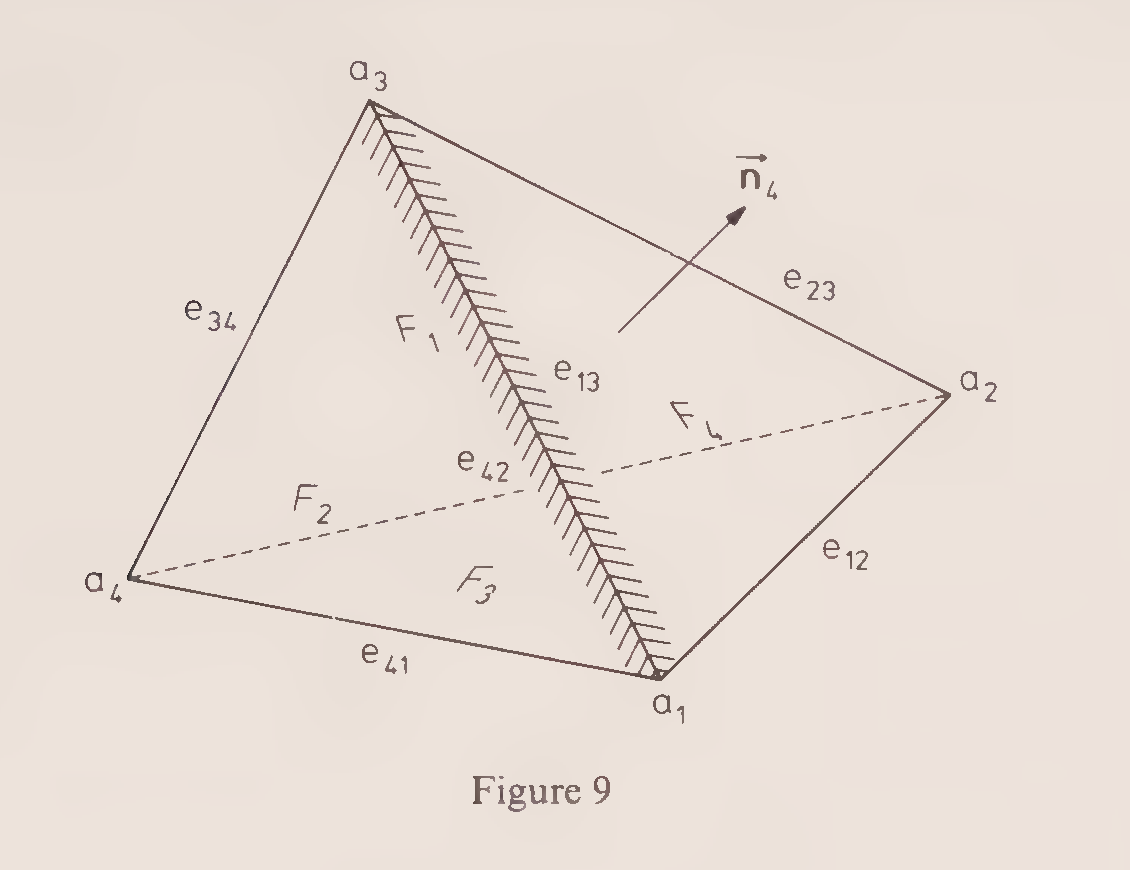
\includegraphics[width=.70\linewidth]{figures/chapter-02-figure-9.png}
\caption{四面体 $\kappa$ 的面、边、顶点和单位外法向量.}
\label{fig:primitive-tetrahedron-geometry}
\end{figure}

公式 \eqref{eq:primitive-bernardi-raugel-bubbles} 和
\eqref{eq:primitive-bernardi-raugel-local-space} 表明, 可以在空间
$\mathcal{P}_1(\kappa)$ 中选取 $\mathbf w$, 其中
\begin{equation}\label{eq:primitive-tetrahedron-first-local-space}
\left\{
\begin{aligned}
\mathcal{P}_1(\kappa)
&=P_1^3\oplus\operatorname{span}
\{\mathbf p_1,\mathbf p_2,\mathbf p_3,\mathbf p_4\}
\subset P_3^3,\\
\mathbf p_1&=\mathbf n_1\lambda_2\lambda_3\lambda_4,
&\mathbf p_2&=\mathbf n_2\lambda_3\lambda_4\lambda_1,\\
\mathbf p_3&=\mathbf n_3\lambda_4\lambda_1\lambda_2,
&\mathbf p_4&=\mathbf n_4\lambda_1\lambda_2\lambda_3.
\end{aligned}
\right.
\end{equation}
注意, $\mathbf p_i$ 在所有 $j\ne i$ 的面 $F_j$ 上消失,
且显然 $\mathbf p_i\times\mathbf n_i=\mathbf0$, 因而
\[
\mathbf p_i\times\mathbf n|_{\partial\kappa}=\mathbf0,
\qquad1\leq i\leq4.
\]
对于 $\mathbf w$ 的自由度, 可以简单地取 $\mathbf w$ 在 $\kappa$
各顶点 $a_i$ 处的值以及它通过各面 $F_i$ 的通量.

Lemma~\ref{lem:primitive-bernardi-raugel-unisolvence} 的论证表明,
这 $16$ 个自由度对 $\mathcal{P}_1(\kappa)$ 唯一可解.

\setcounter{statement}{6}
\begin{Lemma}\label{lem:primitive-tetrahedron-first-unisolvence}
$\mathcal{P}_1(\kappa)$ 中的多项式 $\mathbf p$ 由下列 $16$ 个量唯一确定:
\begin{equation}\label{eq:primitive-tetrahedron-first-dofs}
\left\{
\begin{aligned}
&\mathbf p(a_i),&&1\leq i\leq4,\\
&\int_{F_i}\mathbf p\cdot\mathbf n_i\,\mathrm ds,
&&1\leq i\leq4.
\end{aligned}
\right.
\end{equation}
此外, 在 $\kappa$ 的任意一个面 $F_i$ 上, $\mathbf p$ 只依赖于定义在
该面上的自由度.
\end{Lemma}

相应的速度和压力空间为
\begin{equation}\label{eq:primitive-tetrahedron-first-velocity-spaces}
\left\{
\begin{aligned}
W_h&=\{\,\mathbf w\in\mathcal{C}^0(\bar\Omega)^3;
\ \mathbf w|_\kappa\in\mathcal{P}_1(\kappa)
\quad\forall\kappa\in\mathcal{T}_h\,\},\\
\bar X_h&=W_h\cap H_0^1(\Omega)^3,
\end{aligned}
\right.
\end{equation}
\begin{equation}\label{eq:primitive-tetrahedron-first-pressure-spaces}
\left\{
\begin{aligned}
Q_h&=\{\,q\in L^2(\Omega);
\ q|_\kappa\in P_0\quad\forall\kappa\in\mathcal{T}_h\,\},\\
\bar M_h&=Q_h\cap L_0^2(\Omega).
\end{aligned}
\right.
\end{equation}
